\begin{abstract}
	      This manual shows how to control the Seven Segment Display through the Dabble android application using Wifi in Digital mode and display on the seven segment according the controls in the android app.
\end{abstract}



\subsection{ Connections }
\begin{enumerate}[label=\thesection.\arabic*.,ref=\thesection.\theenumi]
\numberwithin{equation}{enumi}
\numberwithin{figure}{enumi}
\numberwithin{table}{enumi}
\item \textbf{Note} :Components\ref{table:ble-components} and  Connections\ref{fig:vaman/uart/1},\ref{table:ble-connections} are similar to the bluetooth control seven segment display .
\item Now, execute the following code
\item Make sure that change your "ssid","password" in code 
\begin{lstlisting}
vaman/vaman-esp/wifi/codes/src
\end{lstlisting}
\item Build ESP32 firmware
\begin{lstlisting}
cd wifi 
pio run 
\end{lstlisting}
\item Flash ESP32 firmware ( connect Arduino-UART  )
\begin{lstlisting}
pio run -t upload
\end{lstlisting}
\item Now check your mobile/tab is connected with ESP32 
\item Install the wifidabble app
\begin{lstlisting}
vaman/vaman-esp/wifi/wifi_dabble.apk
\end{lstlisting}

\item Open the Dabble application. Enter the vaman Ip adress as shwon in \ref{fig:dabble}
\begin{figure}[H]
\centering
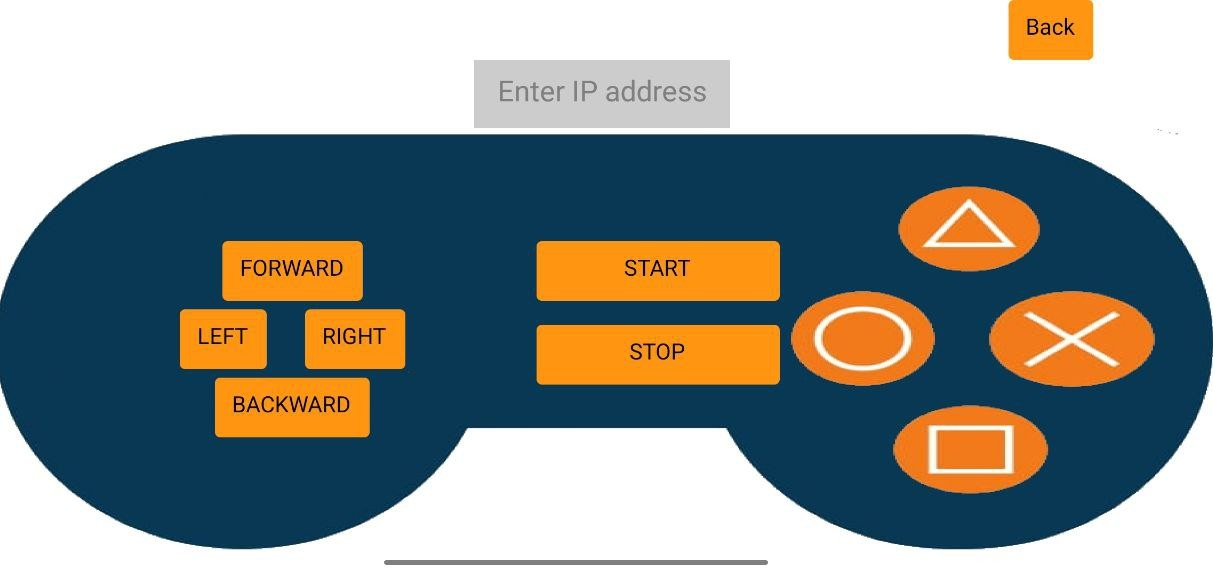
\includegraphics[width=0.6\columnwidth]{figs/wifi.jpg}
\caption{wifi dabble app}
\label{fig:dabble}
\end{figure}
\item Now you can observe the changes on sevensegment display for Start, Up, Down, Right and Left keys pressed on the Digital Mode on the android application
\end{enumerate}